\chapter{The Low Code Development Platform - OpenRefine}\label{ch:the-low-code-development-platform---openrefine}
\section{Overview}
\href{https://openrefine.org/}{OpenRefine} is an application tool that runs locally as a stand-alone application on your computer and uses a web browser
as graphical user interface (GUI). It iss written in \href{https://www.java.com/en/}{Java} and available as open-source and has its roots in managing a knowledge base,
like \href{https://www.wikidata.org/wiki/Wikidata:Main_Page}{Wikidata}. There are other open source alternatives around such as \href{https://workbenchdata.com/}{Workbench}, which follows a similar concept but
is written in Python.~\cite{OpenRefineCoreDump}\\
\newline
OpenRefine can do things such as:
\begin{itemize}
    \item Explore the data by faceting and clustering
    \item Clean messy data e.g. unstructured (or semi-structured) text files
    \item Data transformation, e.g. data normalization and data formatting
    \item Data validation and deduplication
    \item Data reconciliation with external services such as \href{https://www.wikidata.org/wiki/Wikidata:Main_Page}{Wikidata}
    \item Accessing website data for scraping
\end{itemize}

\begin{figure}[H]
    \centering
    
\includegraphics[width=7cm]{./Figures/OpenRefine/openrefine_logo}
    \caption{The OpenRefine Logo}
\end{figure}

\pagebreak
\section{The OpenRefine Graphical User Interface (GUI)}
OpenRefine offers an interactive Graphical User Interface (GUI) that visualizes each step of working with your data set.
It consists of a main grid (or spreadsheet) with the tabular data you are currently working on.

This spreadsheet changes every time you perform an action such as filtering or creating different facets.
The left part of the GUI has a tab for showing each facet/filter that is currently affecting your data set.
This section offers the possibility of quickly changing facets and filters and every time you perform such action,
the spreadsheet reflects the changes.~\cite{OpenRefineCoreDump}\\
\begin{figure}[H]
    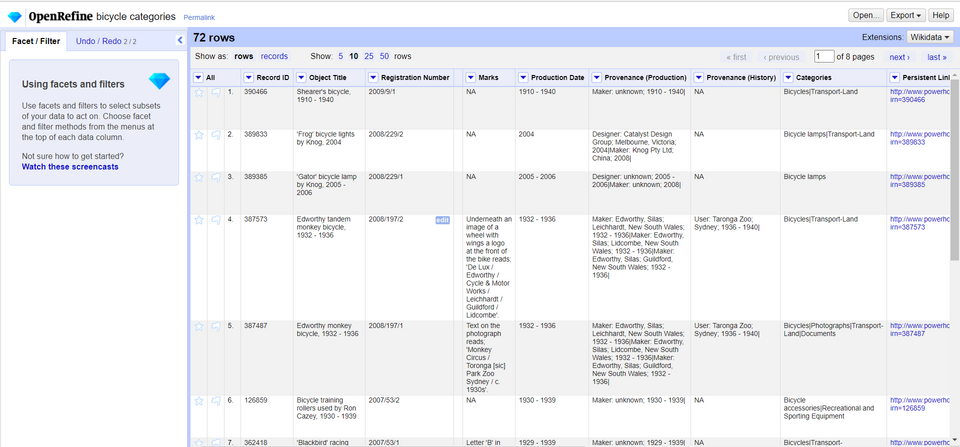
\includegraphics[width=\linewidth]{./Figures/OpenRefine/openrefine_gui}
    \caption{The OpenRefine GUI}
\end{figure}
OpenRefine offers many powerful features such as the \textbf{Undo/Redo} feature or the low coding functions which are essential for efficient bulk data cleaning and transformation.
\pagebreak
\section{OpenRefine Data}
OpenRefine data can come from various sources and usually is initially received as unstructured data. Using OpenRefine, such data is transformed
into well and structured data which can prove to be useful to the user. OpenRefine offers various functions for transformation, cleaning, parsing etc to
transform the data into structured data.
\section{OpenRefine Extensions}
OpenRefine offers an extension architecture for building extensions which extend the functionality of OpenRefine. Some of the extensions are included
into the default OpenRefine installation and the other ones can be manually added to the OpenRefine installation directory. Some of the extensions included
in the official OpenRefine code base are importing Google spreadsheets into OpenRefine, importing database tables into OpenRefine, using the \href{https://www.jython.org/}{Jython}
language for performing functions on the data etc.\\
\newline
In this project, two extensions are built using OpenRefine's extension architecture in order to extend OpenRefine's functionality to
be able to import OpenStreetMap data into OpenRefine (\hyperref[ch:the-osm-extractor-extension]{OSM Extractor}) and also export geospatial
data into the GeoJSON format (\hyperref[ch:the-geojson-export-extension]{GeoJSON Export}).
\section{General Refine Expression Language}
A key feature of OpenRefine is the \textquotedblleft General Refine Expression Language \textquotedblright, or GREL.
GREL is an expression language specific to OpenRefine, which is similar to JavaScript and is convenient for performing different functions such as:
\begin{itemize}
    \item String operations
    \item Boolean operators
    \item Parsing HTML, JSON or XML
    \item Selecting HTML elements
    \item Iterating over elements etc.
    \item GREL is going to be used in our case to access the HTML DOM and
    \item select the appropriate data out of the HTML page for scraping.
\end{itemize}~\cite{OpenRefineCoreDump}\\
\newline
One of the extensions of this project includes adding a new GREL function called \mintinline{java}{interiorPoint()}
which serves as a function to compute the interior point of a Geometry.